\documentclass[12pt]{article}
\oddsidemargin -0.5in
\evensidemargin -0.5in
\textwidth 7.2in
\topmargin -0.5in
\textheight 8in
\flushbottom

\usepackage[authoryear,round]{natbib} %a package for formatting citations
\usepackage{amsmath} %a package for good looking equations and symbols
\usepackage{algorithm2e} %a package for typesetting algorithms
% \usepackage{caption} %a package for more complex captions for figures/tables/images
\usepackage{subcaption} %extension of the caption package
\usepackage{url} %embedded, clickable links
\usepackage{fullpage} %including this package changes the default margins to use more of the page
\usepackage{graphicx} %package for inline images
\usepackage[usenames]{xcolor} %for adding color text
\usepackage{enumitem} %for nested numbered lists (like in the questions section)
% \usepackage{hyperref}
% \usepackage{amsfonts}

\newcommand{\nextproblem}{
	\vfill
	\pagebreak
}
% \setlist[itemize]{noitemsep, topsep=0pt}
\graphicspath{{plots/}}

\begin{document}


	\begin{center}
			\textbf{CS 4641 Machine Learning} \vspace*{2mm}
			\textbf{\\ Bojun Yang | Section B} \vspace*{2mm}
			\textbf{\\ Homework 2 Writeup }
	\end{center}
	% \vspace*{2mm}


\begin{enumerate}[noitemsep,topsep=0pt]
\item KNN Analysis
\begin{enumerate}
    \item Euclidean Distance
    \\ 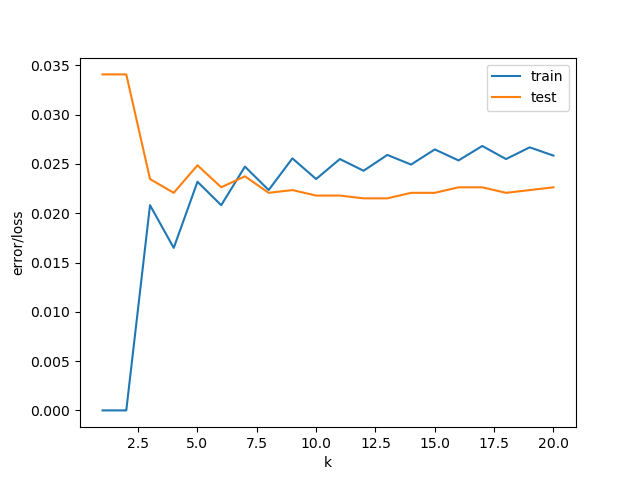
\includegraphics[height=0.4\textheight]{HTRU2_euc}
    \item Manhattan Distance
    \\ 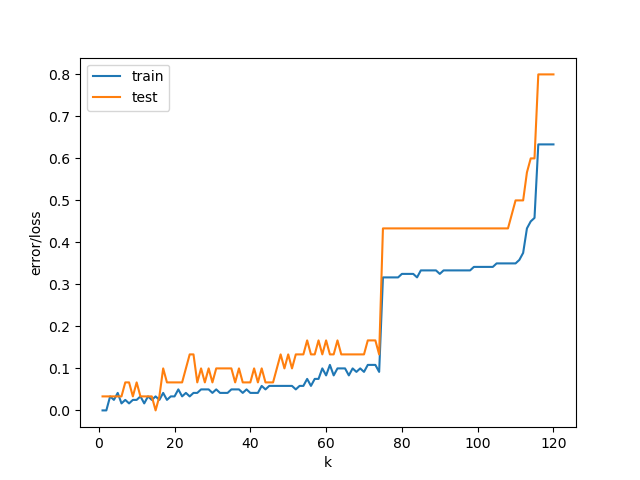
\includegraphics[height=0.4\textheight]{iris_euc}
    \item Mahalanobis Distance
    \\ 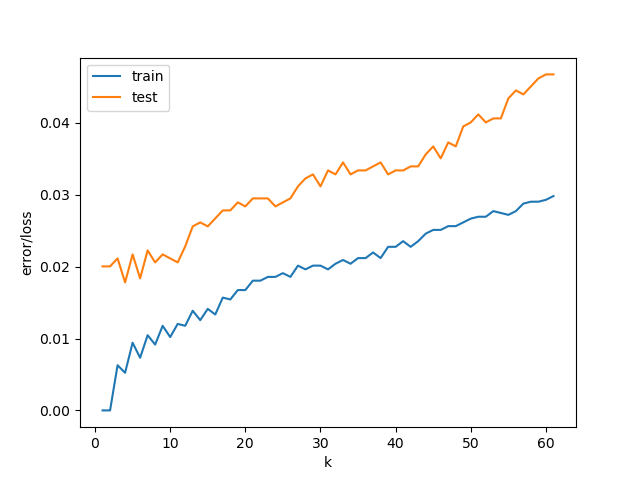
\includegraphics[height=0.4\textheight]{digits_euc}
\end{enumerate}


\end{enumerate}

\end{document}

